\newpage
\section{Objetivos}

Nesta prática analisaremos alguns processos térmicos em gases, utilizando experimentos diversos para medir alguns parâmetros. Primeiramente, nos dois experimentos iniciais, vamos buscar encontrar o valor do fator $\gamma$ do ar, que pode ser definido como a razão entre os calores específicos a pressão e a volume constantes ($\gamma$ = $c_p/c_v$). Vamos utilizar os métodos de Clément-Desormes (1º experimento) e de Ruchardt (2º experimento) para obter tal constante. Para o 3º experimento, vamos determinar a temperatura de zero absoluto utilizando um termômetro de gás a volume constante.\\

Assim, a prática envolverá diferentes processos térmicos em gases, com os quais buscaremos entender melhor esse escopo da termodinâmica.\\

\begin{figure}[H]
  \centering
  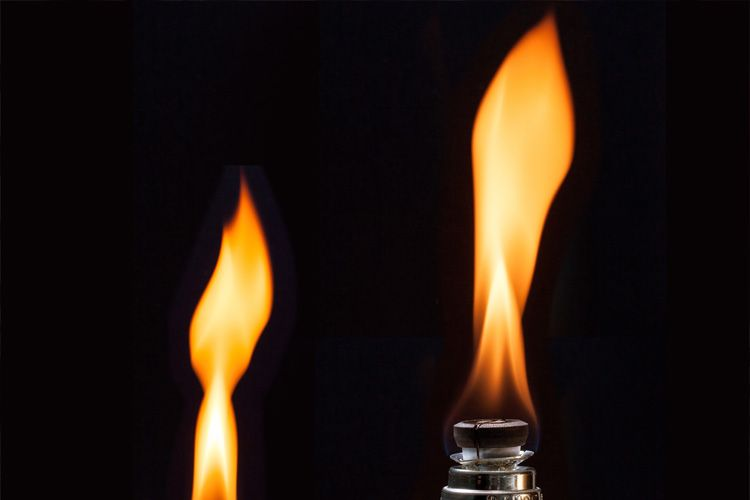
\includegraphics[scale=0.5]{images/termodinamica.jpg}
  \caption{Um exemplo de reação estudada pela termodinâmica: a combustão.}
\end{figure}
